\chapter{Introduction}

On June 2, 2016, a bright object could have been observed streaking through the night sky of Arizona. 
This object caused sonic booms to occur over the area of Phoenix AR, and reports of this bright object were taken from California, Colorado, Texas, Utah, New Mexico, and Nevada [\cite{palotai2018analysis}]. 
This is not the first nor last time that an object of this nature will occur in the continental United States, with a more extreme version of this event having occurred in Tunguska in 1908\cite{PBrown2002}.

Just what were these objects that can come streaking in with a brilliant magnitude of light? 
For that, we must look beyond the Earth's atmosphere and into the neighborhood of the solar system. 
Where, accompanied by the planets and the sun, are many bits of rock and ice swirling around, some creating swarms that we have nicknamed for when they impact the Earth's atmosphere. 
These bits of dust and rock are termed either asteroids or meteoroids, depending on their size, as seen in figure 1. 

The concern of this paper however, is on the meteoroids that end up colliding with the Earth's atmosphere, termed meteors, which when impacted the atmosphere, begin to ablate, or burn up, on collision with the air molecules. 
Without this sphere of atmosphere of course, all of those meteoroids would impact the ground directly, which would be rather catastrophic to human society as a whole. 
As it is, the ablation of the meteor due to friction from the air molecules causes it to ignite, releasing light and heat into the atmosphere, which is what is observed from the ground.

To capture images of these fireballs, there are many different kinds of camera setups that will be discussed in more detail further into the paper. For now, our attention will be turned to the Willamette D6 AllSky Cam-
era, which operates rather differently from most mainstream methods of fireball detection. 
Being the size and shape of a short parking bollard, it can easily be picked up and moved to whichever location is deemed to best fit the needs of detection. 
An added bonus being that there is no super computer involved, just a small microprocessor that uses the camera to view the night sky. 
Only taking captures when the parameters for fireball occurrences are met so as to save space as well as save time when perusing through and analysing the data.

The data being collected can include how long the fireball is observed, the level of brightness it lets off, and other factors, the energy of the fireball can be calculated, known as the optical energy. 
Peter Brown is an astronomer who found a link between the optical energy of a fireball and the flux, which is an estimate of the density of a given fireball with a certain optical energy. 
Or in other terms, given the optical energy of a fireball, and using Peter Browns method, it can be determined how many of that type of fireball will collide with the Earth's atmosphere in a given year.

This project will be focused on investigating if the Willamette D6 AllSky Camera, hereby referred to as D6, is an effective alternative for fireball detection. 
This will be done by comparing our fireball flux graphs to those given by Peter Brown in his paper, =with an example being shown in figure 2.2. 
Comparing our results to those found in figure 2.2 will give us an idea of how close the data being received by D6 is to the data received by more established methods.




\begin{figure}
    \centering
    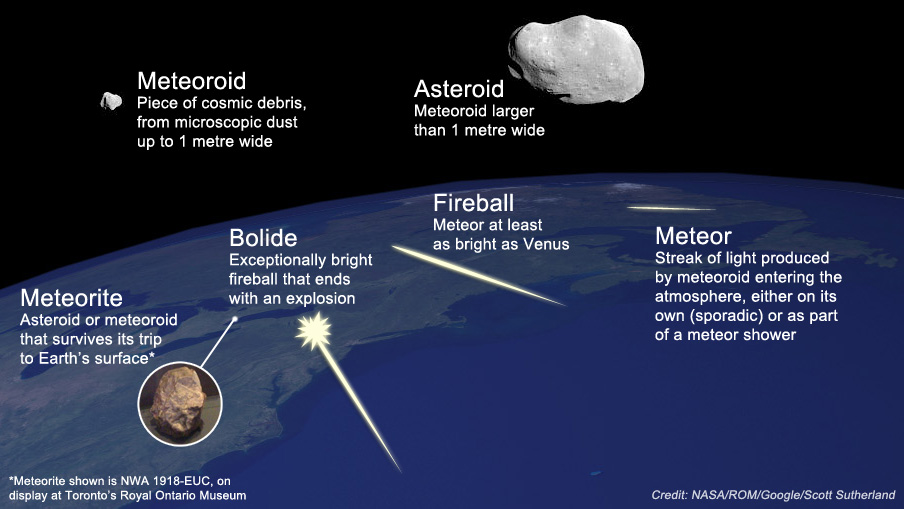
\includegraphics[width=10cm]{Meteor_comparison.png}
    \centering
    \caption{Graphical Overview of the different kinds rock floating around the solar system. As can be seen, an asteroid is much larger than a meteoroid, and there are many sub-branches of a meteor once it is in the atmosphere.}
    \label{fig: 1.1}
\end{figure}

\begin{figure}
    \centering
    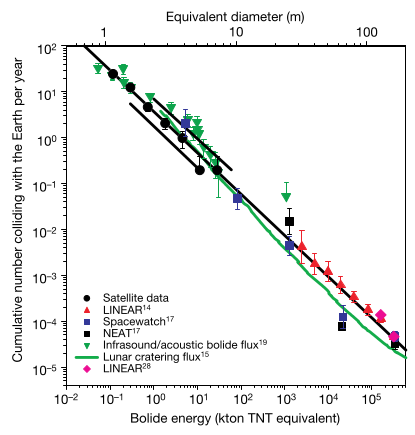
\includegraphics[width=8cm]{flux_brown.png}
    \centering
    \caption{Graph of Flux numbers, which is the number of meteoroid types colliding with the Earth by their energy. This graph will be useful when we start analysing our data to determine if D6 is a good alternative to other detection systems.}
    \label{fig: 1.2}
\end{figure}
